\chapter*{Method}

This chapter will describe how the research is executed and which elements that is used. All Hardware, software and processes used will be described to increase the repeatability and validity of the research. The research can be divided into three, lab environment design and tests, traffic capturing and traffic analysis.

\section{Testing}
Testing is done in three different phases in this master thesis, this structure will allow the results from the previous testing to be used in the later phases and produce more accurate results.

    \paragraph{Phase 1: } In this phase the lab environment is setup and live for some time. When the setup is stable the stand by traffic test is executed. 

    \paragraph{Phase 2: } At this point we define six different event tests to be executed by the robot vacuum cleaner and captured. All tests are done a defined number of times, in two different test environment. 

    \paragraph{Phase 3: } The last phase is evaluation testing. The robot vacuum cleaner is deployed in three different environment, where other smart home devices are connected to the same local area network. 

\subsection{Phase 1: Initial testing}
Smart home environment is configured and verified in the created lab. The vacuum cleaner does home discovery, during this process the vacuum cleaner is moving around and mapping all available floors, with fruiterers.reference maybe. The lab environment is configured according to table x-x, and connected as figure x shows.

\subsubsection{Capturing platform}
A Raspberry PI 3b+ is used as the capturing platform during this mater thesis. The platform is small, autonomous and can be configured to do complex tasks in similar environments, \cite{Raspberrypi3_as_a_platform} and \cite{Raspberrypi3_as_a_platform_1} has implemented sensor and wireless sniffing on this device. It has one ethernet RJ-45 port and a wireless IEEE.802.11 NIC integrated, this enables both LAN and WLAN sniffing at the same time. 

\begin{table}[!hbtp]
\centering
\caption{Capturing platform}
    \begin{tabular}{|l|l|}
    \hline
    Device           & Raspberry Pi3 b+     \\ \hline
    OS               & Kali Linux, Version? \\ \hline
    Tshark           & Version?             \\ \hline
    Wireshark        & Version?             \\ \hline
    External device  & Wi-Fi adapter        \\ \hline
    External storage & Micro SD-card 32Gb   \\ \hline
    \end{tabular}
\end{table}

\subsubsection{Local area network switch}
The local area network switch is used to duplicate the bidirectional network traffic from the access point, to the LAN NIC in the capturing platform.  This is done with the a SPAN port configuration, shown in figure XX \cite{Network_Span_port}.An Cisco Catalyst 2960 switch \cite{cisco_catalyst_8_port} is used based on its SPAN port support, and availability. 

\begin{table}[!hbtp]
\centering
\caption{Local area network switch}
    \begin{tabular}{|l|l|}
    \hline
        Device & Cisco Catalyst 2960 \\ \hline
        OS     & IOS version?        \\ \hline
    \end{tabular}
\end{table}

\subsubsection{Access point}
An Access point is added to the smart home lab environment, and broadcasts one SSID. To make the capturing attribution more accurate the SSID is only broadcaster on IEEE 802.11 channel 1. If not some packets can be missed due to channel hoping. Configuration overview is shown in figure XX. 

\begin{table}[!hbtp]
\centering
\caption{Access point}
    \begin{tabular}{|l|l|}
    \hline
        Device & TP-Link Access point \\ \hline
        OS     & IOS version?         \\ \hline
    \end{tabular}
\end{table}

\subsubsection{Baseline network traffic capture}
At the end of phase one, the standby network traffic capture is done. During the baseline network traffic capture, there is no events triggered on the robot vacuum cleaner. Baseline traffic will represent the traffic which is not generated due to events triggered and can be filtered away. 

\section{Traffic capturing}
Smart home devices often generates network traffic continuous, as robot vacuum cleaners are cloud based they need to establish and keep alive a secure tunnel where commando and control can be executed. This section will describe how the captures are done and extracted to the location where the packet captures will be analysed. 
- Capturing in files

- Tshark filter

- Defining files




\section{Traffic Analysis}
To ensure that the research will produce the best contribution to the field of information security. Several different analysis tools will be used, but the main focus will be to use the best satiable machine learning algorithm for this purpose. The Traffic analysis section of this method will include the selection of there methods and, ect    

\section{Smart Home Environment}
To be able to perform passive eavesdropping on a robot vacuum cleaner there have to be set up a lab environment which is able to act similar as a normal smart home environment and allow the traffic and events to be controlled. This parts include the selection of smart home environment, it also includes the selection of devices to use such as robot vacuum cleaner, sniffing hardware and software as well as network design to allow capturing of traffic is the different phases in smart home communication. 

\subsection{Apartment}
The smart home environment will be set up in an apartment in Oslo, the whole apartment is 85m2 and the cleaning area of will be limited to the living room with 12m2. This is illustrated in figure XX. The apartment is located in the 4th floor of a brick building which have a 5th floor. This apartment is chosen because the author of this thesis lives here and it will therefore be a representative live smart home environment.

\begin{figure}[!ht]
    \centering
    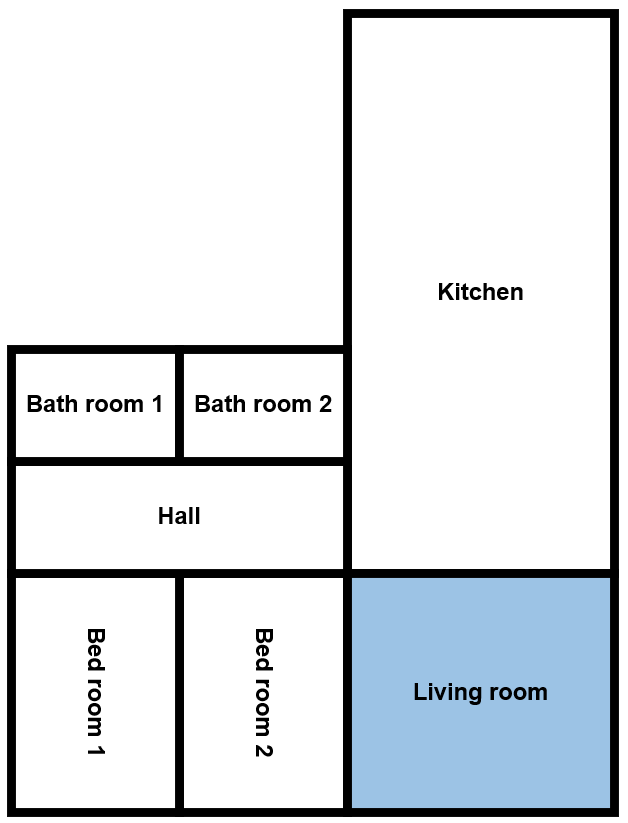
\includegraphics[width=10cm]{figures/Apartment.png}
    \caption{Network High Level Design}
    \label{fig:HLD}
\end{figure}

 The living room is 3,30m x 3,64m and aprox 12 m2. and includes furniture as shown in the figure XX. 

\begin{figure}[!ht]
    \centering
    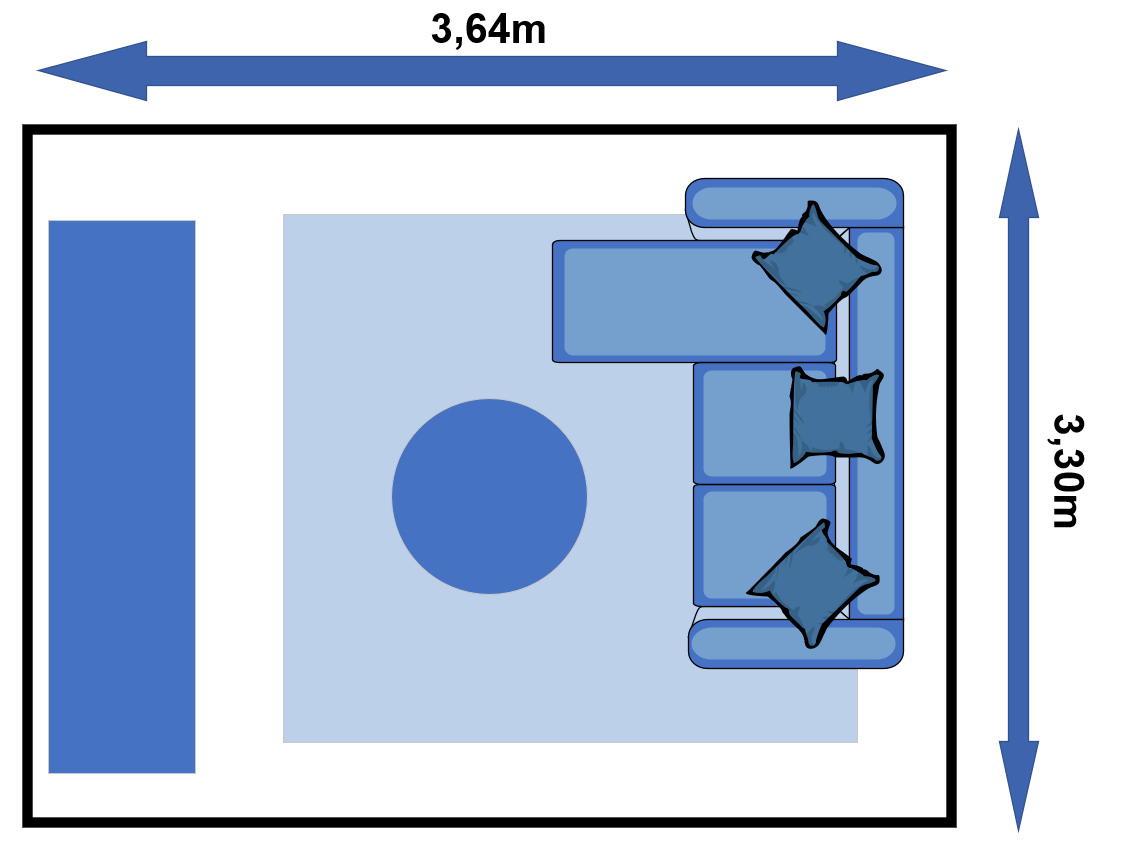
\includegraphics[width=10cm]{figures/Living room.png}
    \caption{Network High Level Design}
    \label{fig:HLD}
\end{figure}

\subsection{Robot vacuum cleaner}
The robot vacuum cleaner is the main device in this research. To select the best suited vacuum cleaner we did a selection survey which based on the requirements we had about different smart home features, price, norwegian distributor and popularity. The survey selected resulted in Irobot roomba 7i as the best option. The selection process and secifications for Irobot roomba i7 is described in subsections below.

\subsubsection{Robot vacuum selection}
Because of limited resources and time, the selection of equipment needs to be done before acquiring anything. The vacuum will need several smart home features so that the different features can be identified in the network traffic analysis. The purpose of this research is to identify how much private information which can be gathered as well as how complex these types of sniffing attack will have to be. Selecting a vacuum cleaner with more smart home features will potentially reveal more sensitive private information.

    \paragraph{Communication network protocols:} IoT devices can use several different network protocols and technology to communicate with other devices. We distinguish between Datalink layer (layer 2), Network layer (layer 3), session layer (layer 4) and Application layer (layer 5). Each of these layers can reveal different information about the session, devices and data which is sent. The Data Link Layer protocol IEEE 802.11 (Wi-Fi) it is the most widespread infrastructure in smart homes \cite{robotsel1}. Wi-fi will therefore be the preferred data link layer protocol, this to ensure the most relevant result \cite{robotsel2}\cite{robotsel3}. The selection of IEEE 802.11 will result in more common Internet routing protocols which supports the principle.

    \paragraph{App features:} To enable the best user experience possible more and more IoT devices comes with dedicated application for command, control, statistics, and integration. Such applications add new smart home features to devices which often result in more data transfers between the device and the cartelized controller. The application architecture is dependent on the vendor, but a common design is a client-server architecture, where both the vacuum cleaner and mobile application is acting as clients \cite{robotsel4}. This may include sensitive private information transferred between the devices. \cite{robotsel7}

    \paragraph{Navigation:}A robot vacuum cleaner will have to navigate around the smart home to be able to clean sufficiently. This navigation is handled differently, form the basic to more advanced navigation. Some of the more advances navigation systems uses laser or camera to navigate and map the environment. \cite{robotsel5} \cite{robotsel6} This type of mapping could generate some interesting information for the research. 

\paragraph{}Open-source information, tests sites and YouTube videos are used to gather information to base the selection on. To limit the number of relevant robot vacuum cleaner vendors I used open source review sites to determine which vendors that had the highest ranking robots. Next, I used Google Play and the available statistics to see how many downloads and rating the different vendor specific application had. Based on the results from these findings I filtered the vendor models based on app features and navigation described in the introduction, the best suited robot vacuums per vendor is then compared to each other to finally select one. Prices are gathered from the comparison website prisjakt.no\cite{prisjakt.no}. 

 From opensource test sites there was two robot vacuum vendors which did good, Irobot and Roborock, these are therefore the main vendors to be considered. As reference to another popular vendor Xiaomi is also included in the survey.\cite{robotsel11}\cite{robotsel12}\cite{robotsel13}

\paragraph{Selection:} \cite{robotsel11}\cite{robotsel12}\cite{robotsel13} is used as vendor comparison review sites, these were selected because they were some of the top results on my google with the search string “Robot vacuum cleaner test”. The vendor on top ten selection \cite{robotsel11} is listed in tabel XX, \cite{robotsel12} listed in tabel XX and \cite{robotsel13} listed in tabel XX. 

\begin{table}[]
\begin{tabular}{|l|c|}
\hline
Vendor   & Number on top ten \\ \hline
Roborock & 3                 \\ \hline
Irobot   & 3                 \\ \hline
ILife    & 2                 \\ \hline
Wyze     & 1                 \\ \hline
Neato    & 1                 \\ \hline
\end{tabular}
\end{table}


\begin{table}[]
\begin{tabular}{|c|c|}
\hline
Vendor    & Number on top ten \\ \hline
Ecovacs   & 2                 \\ \hline
Irobot    & 2                 \\ \hline
Roborock  & 2                 \\ \hline
Shark     & 1                 \\ \hline
Eufy      & 1                 \\ \hline
ILife     & 1                 \\ \hline
Proscenic & 1                 \\ \hline
\end{tabular}
\end{table}

\begin{table}[]
\begin{tabular}{|c|c|}
\hline
Vendor   & Number on top ten \\ \hline
Irobot   & 2                 \\ \hline
Roborock & 2                 \\ \hline
Neatsvor & 3                 \\ \hline
Ecovacs  & 1                 \\ \hline
Neato    & 1                 \\ \hline
Kyvol    & 1                 \\ \hline
\end{tabular}
\end{table}

\begin{table}[]
\begin{tabular}{|c|c|}
\hline
Vendor    & Number on top ten \\ \hline
Irobot    & 7                 \\ \hline
Roborock  & 7                 \\ \hline
Neatsvor  & 3                 \\ \hline
Ecovacs   & 3                 \\ \hline
ILife     & 3                 \\ \hline
Neato     & 2                 \\ \hline
Proscenic & 1                 \\ \hline
Wyze      & 1                 \\ \hline
Shark     & 1                 \\ \hline
Eufy      & 1                 \\ \hline
Kyvol     & 1                 \\ \hline
\end{tabular}
\end{table}

To get a briefly overview of the popularity of the different robot vacuum cleaners we can use the number of downloads of the different applications. This information is available in Google play with overall user rating, application rating is also available in Apples App Store. 

\begin{table}[]
\begin{tabular}{|c|c|c|}
\hline
Application & Google play download & App rating 0-5 \\ \hline
Irobot      & 5 million+           & 4,0            \\ \hline
Roborock    & 1 million +          & 4,6            \\ \hline
Xiaomi      & 10 million +         & 4,3            \\ \hline
Ecovacs     & 1 million +          & 2,5            \\ \hline
Shark       & 1 million +          & 3,3            \\ \hline
Eufy        & 1 million +          & 4,6            \\ \hline
ILife       & 10 thousand +        & 2,2            \\ \hline
Wyze        & 1 million +          & 4,0            \\ \hline
Proscentic  & 100 thousand +       & 2,0            \\ \hline
\end{tabular}
\end{table}

As we can see the most downloaded applications in google play is “Irobot” and “Xiaomi”, the difference between these two applications is that Irobot is a pure vacuum cleaner application and Xiaomi is a smart home application where you can connect other IoT devices and control your integrated smart home.  
Satisfaction based on rating is also divided between the different application, applications with the rating above 3.9 is: Irobot, Roborock, Xiamoi, Eufy and Wyze. 

\paragraph{Discussion} Based on the open-source top ten site review the results showed that Irobot and Roborock was the overall best vendors on the marked. These are therefore the most relevant vendors to compare to find the most suited vacuum cleaner to our project. This assumption is also supported when it comes to the results from Google play statistics, there we can see that both Irobot and Roborock is among the highest rated and downloaded applications. These two results make us confident that a vacuum cleaner from one of these vendors will give us a popular and well used vacuum cleaner which makes the research results more relevant. 
Xiaomi is the most downloaded application in Google play with more than 10 million downloads, in difference with the applications from iRobot and Roborock the application is designed to handle an entire smart home and not just vacuum cleaners. As Xiaomi has a lot of other IoT devices on the marked this could cause more downloads which is not directly connected to the use of their vacuum cleaners. Is was also not mentioned in any of the top ten review sites which we used and is therefore not the right fit for this research. If the purpose was to analyse an entire smart home, it could be more relevant due to the integration features in the smart home application. 
Most suitable vendor vacuum: 
Irobot Roomba I7 is the most suitable model from Irobot in this research project. This is the model which includes all the smart features included through the app without extra cost associated with extra cleaning features. Compared to the I6 model I has newer hardware and support for minimal cost. \cite{robotsel9}

\paragraph{Conclution} Both iRobot Roomba i7 and Roborock has a lot of the same features which is must have on a robot vacuum cleaner, as well as they are in the same price range. The advantage of 5 million downloads vs Roborock’s 1 million indicated that the iRobot vacuum cleaners are more used combined with smart home features. The iRobot also has seasonal and pet detection and can make suggestions on the cleaning patters, this ability to identify user behaviour could create a lot of sensitive private information about it’s roommates. iRobot Roomba i7 will therefore be the most suitable robot vacuum cleaner for this research




\subsubsection{Network design}
To represent the general smart home in common homes the research used the existing network infrastructure in the apartment and added some components to be able to better isolate the traffic from the robot vacuum cleaner. The different elements are show in figre \ref{fig:HLD}, further each device will be described. 

\begin{figure}[!ht]
    \centering
    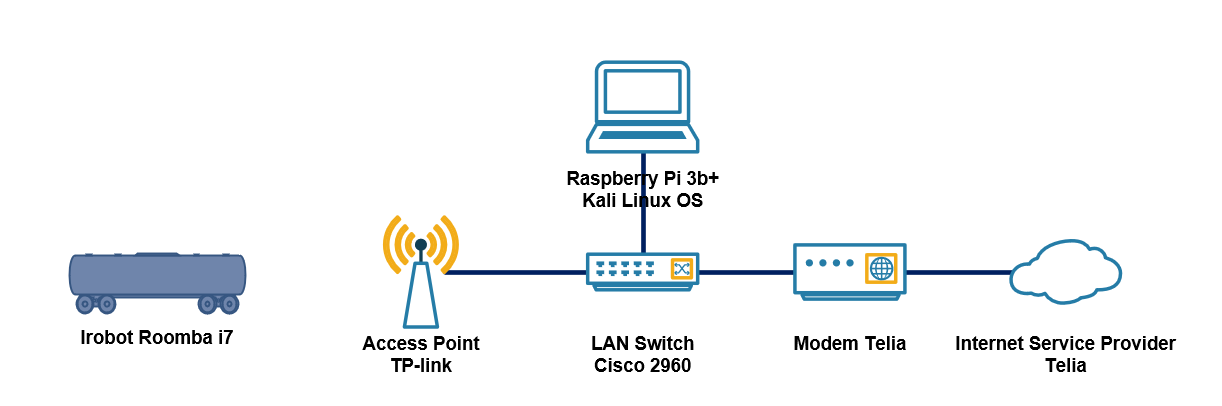
\includegraphics[width=10cm]{figures/HLD.png}
    \caption{Network High Level Design}
    \label{fig:HLD}
\end{figure}

\begin{itemize}
    \item \textbf{Device:} Raspberry Pi 3b+
    \item \textbf{Software:} Kali ARM \cite{kalidownload}, updated 27.09.2022
    \item \textbf{Configuration:}
    \begin{enumerate}
        \item Image downloaded to an external computer and written to the micro SD-card with the application balenaEtcher \cite{balenaetcherdownload}.
        \item Patching done 19.12.2022 with the command "sudo apt update \&\& sudo apt upgrade"
    \end{enumerate}
    \item \textbf{Connected items:}
    \begin{enumerate}
        \item Micro SD card \cite{microsdcard}
        \item TL-WN722N USB WiFi Adapter \cite{tp-link}
    \end{enumerate}
\end{itemize}

\section{Test cases}
Each test Case consists of a detailed test description, which enables the tests and results to be reproduced as identical as possible. It will also state how many times the test was done during the research. The standby traffic test is performed over 14 consecutive days, and all other tests are done 20 times. The number of days and tests are decided based on the available time frame for this master thesis. Equipment selection process, design and configuration process and test phase is time consuming and 20 is therefore chosen as the overall test number. 

\subsection{Baseline-traffic}
Baseline test have the function to represent the traffic flow generated by the robot vacuum cleaner installed in the smart home environment with out any event triggering. For this test the robot vacuum cleaner is installed in the chosen smart home environment described in "smart home environment chapter". Before the test was conducted the robot was operational for more then 60 days, and more then 10 cleaning jobs done. This to ensure that is is in operational mode.

\begin{itemize}
    \item \textbf{Description:} Conduct packet sniffing for both wireless and cabled traffic generated over a number consecutive days. Capture data is stored in two separate files. The Robot vacuum cleaner is connected to power and Internet the entire time period.
    \item \textbf{Number of tests:} 14 consecutive days
\end{itemize}

\subsection{Triggered cleaning}
Triggered cleaning is an event started trough the IRobot application with the use of "start cleaning". The test is done when the mobile application receives a notification that the cleaning is done. If the robot vacuum need to return to base to recharge, empty bin or get stuck something in the brushes, actions will be done to enable the robot to continue cleaning. 
\begin{itemize}
    \item \textbf{Description:} Start cleaning through the Irobot application, with the use of start cleaning. Capture is started 10 minutes before cleaning is scheduled and stopped 30 minutes after the cleaning is finished. 
    \item \textbf{Number of tests:} 20
\end{itemize}

\subsection{Empty bin} The bin needs to be removed from the vacuum cleaner to be emptied. This will make the vacuum cleaner in a state where is cannot start cleaning, and the application will display information about the situation. 

\begin{itemize}
    \item \textbf{Description:}Start packet capturing 5 minutes before the bin is removed. Remove the bin, wait 5 minutes and then insert the bin once more. Stop capturing 5 minutes after the bin is inserted
    \item \textbf{Number of tests:}20
\end{itemize}

\subsection{Open mobile application}
Mobile application will be able to access information about the robot vacuum cleaner. This might generate pull requests from the Irobot cloud towards the vacuum cleaner to get the needed information to display. If the user changes attribute in the application this needs to be communicated with the vacuum cleaner. 
\begin{itemize}
    \item \textbf{Description:} Start packet capturing 5 minutes before opening the application on the smart phone. Open the application, change a "room name" and one "room separation line", then wait until the application have been open for 5 minutes, then close the application. Stop packet capturing after additionally 5 minutes. 
    \item \textbf{Number of tests:}20
\end{itemize}



\section{Methods in relates work}
Through some one the papers review in the related work section they used to capture live traffic from the smart devices.In this section the different methods in \cite{lindaeavesdropping} \cite{eavsIoT} \cite{Neato}, will be discussed and elements that could be used in this research will be identified and justified. 


\begin{itemize}
    \item \textbf{Description:}
    \item \textbf{Number of tests:}20
\end{itemize}